\documentclass[9pt,twocolumn,twoside,lineno]{pnas-new}
% Use the lineno option to display guide line numbers if required.

\usepackage{todonotes}
\usepackage{biblatex}
\addbibresource{references}

\newcommand\focalcountry{CHE}
\newcommand\mindate{01. Jan. 2020}
\newcommand\maxdate{01. Dec. 2020}
\newcommand\maxmissing{2903}
\newcommand\minlength{27000}
\newcommand\maxsamplingfraction{0.05}
\newcommand\subsamplebycanton{TRUE}
\newcommand\travelcontextscalefactor{0}
\newcommand\similaritycontextscalefactor{2}
\newcommand\traveldataweights{1,1,1}
\newcommand\whichtrees{\.*}
\newcommand\pickchainsunderothercriteria{TRUE}
\newcommand\ntrees{-1}
\newcommand\smoothconfcases{FALSE}
\newcommand\outgroupgisaidepiisls{EPI\_ISL\_406798}
\newcommand\uniquecontextonly{FALSE}
\newcommand\maskfromstart{100}
\newcommand\maskfromend{50}


\templatetype{pnasresearcharticle} % Choose template 
% {pnasresearcharticle} = Template for a two-column research article
% {pnasmathematics} %= Template for a one-column mathematics article
% {pnasinvited} %= Template for a PNAS invited submission

\title{SARS-CoV-2 Genome surveillance in Switzerland: Can we quantify the effects of policy?}

% Use letters for affiliations, numbers to show equal authorship (if applicable) and to indicate the corresponding author
\author[a,c,1]{Author One}
\author[b,1,2]{Author Two} 
\author[a]{Author Three}

\affil[a]{Affiliation One}
\affil[b]{Affiliation Two}
\affil[c]{Affiliation Three}

% Please give the surname of the lead author for the running footer
\leadauthor{Lead author last name} 

% Please add a significance statement to explain the relevance of your work
\significancestatement{Authors must submit a 120-word maximum statement about the significance of their research paper written at a level understandable to an undergraduate educated scientist outside their field of speciality. The primary goal of the significance statement is to explain the relevance of the work in broad context to a broad readership. The significance statement appears in the paper itself and is required for all research papers.}

% Please include corresponding author, author contribution and author declaration information
\authorcontributions{Please provide details of author contributions here.}
\authordeclaration{Please declare any competing interests here.}
\equalauthors{\textsuperscript{1}A.O.(Author One) contributed equally to this work with A.T. (Author Two) (remove if not applicable).}
\correspondingauthor{\textsuperscript{2}To whom correspondence should be addressed. E-mail: author.two\@email.com}

% At least three keywords are required at submission. Please provide three to five keywords, separated by the pipe symbol.
\keywords{Keyword 1 $|$ Keyword 2 $|$ Keyword 3 $|$ ...} 

\begin{abstract}
% Please provide an abstract of no more than 250 words in a single paragraph. Abstracts should explain to the general reader the major contributions of the article. References in the abstract must be cited in full within the abstract itself and cited in the text.
Are the effects of policies designed to prevent and contain SARS-CoV-2 imports evident in genomic surveillance data? Here we use SARS-CoV-2 genome sequences from approximately \totalsamplingpercent\% of all confirmed cases in Switzerland from the first case on 25. Feb. through \maxdate\ to identify local transmission chains and quantify their spread in Switzerland. We first performed a large-scale phylogenetic analysis to characterize the dynamics of virus imports into Switzerland. We then performed a phylodynamic analysis to quantify transmission chain spread in Switzerland and test whether Switzerland’s contact tracing program was able to slow the spread of imported lineages once local cases were identified. These analyses aim to help us understand the importance of international travel towards a national epidemic, an increasingly relevant topic as global vaccination campaigns continue at an uneven pace and new variants of concern spread internationally.
\end{abstract}

\dates{This manuscript was compiled on \today}
\doi{\url{www.pnas.org/cgi/doi/10.1073/pnas.XXXXXXXXXX}}

\begin{document}

\maketitle
\thispagestyle{firststyle}
\ifthenelse{\boolean{shortarticle}}{\ifthenelse{\boolean{singlecolumn}}{\abscontentformatted}{\abscontent}}{}

% \subsection*{Author Affiliations}

% Include department, institution, and complete address, with the ZIP/postal code, for each author. Use lower case letters to match authors with institutions, as shown in the example. PNAS strongly encourages authors to supply an \href{https://orcid.org/}{ORCID identifier} for each author. Individual authors must link their ORCID account to their PNAS account at \href{http://www.pnascentral.org/}{www.pnascentral.org}. For proper authentication, authors must provide their ORCID at submission and are not permitted to add ORCIDs on proofs.

\section{Introduction}
% If your first paragraph (i.e. with the \dropcap) contains a list environment (quote, quotation, theorem, definition, enumerate, itemize...), the line after the list may have some extra indentation. If this is the case, add \parshape=0 to the end of the list environment.
% \dropcap{T}his PNAS journal template is provided to help you write your work in the correct journal format. Instructions for use are provided below. 

% Claim importance
\dropcap{P}ublic health policies must prevent or break transmission chains to stem an epidemic, but case-level data to investigate individual transmission chains, and the effect of interventions on their spread, is often lacking. These data are both difficult to collect and sensitive. In the absence of contact tracing data, pathogen genomes provide an alternate source of information on the relationships between cases in an epidemic. As viruses replicate and spread, they accumulate mutations in their genetic code. Given a sufficiently fast-mutating virus, one can estimate which cases in an outbreak are from the same transmission chain based on shared mutations in the infecting viruses. 

% During the SARS-CoV-2 pandemic, viral genome data have been generated and analyzed at unprecedented speed and scale. First, SARS-CoV-2 genomes collected from some of the first confirmed cases in late December 2019 and early January 2020 were all very genetically similar, suggesting the origin of the pandemic was a single zoonotic jump of the virus from animals into humans around November 2019 \cite{VirologicalRambaut}.  
% Then, as SARS-CoV-2 spread from China - where it was first identified - and began to diversify, comparison of early cases in new regions helped establish when local transmission began, e.g. \cite{Worobey2020a}.
% Finally, in Summer and Fall 2020, genome surveillance helped identify, investigate, and track mutations suspected of conferring increased transmissibility, increased pathogenicity, or vaccine escape, e.g. \cite{Hodcroft2020Emergence14, Rambautb}.

SARS-CoV-2 genome data have been extensively used to characterize and quantify aspects of regional COVID-19 epidemics and their composite transmission chains. One common approach involves constructing a phylogenetic tree from viral genomes that represents the relationships between cases. Specific events, like imports from abroad, super-spreading events, and spread along a transmission chain can be inferred based on the clustering of cases in the phylogeny, e.g. \cite{Lu2020, Eden2020, OudeMunnink2020, Bluhm2020}. Going one step further, more complex phylodynamic analyses fit an epidemiological model to the phylogeny where branching times (transmission events) are explained by epidemiological parameters \cite{Grenfell2004}.  

Importantly, these phylogenetic and phylodynamic methods can help evaluate the effects of public health policy on epidemic spread. For instance, \cite{Mallon2020, duPlessis2021} showed that major reductions in lineage diversity and size or geographic distribution of lineages in the Irish and English SARS-CoV-2 epidemics coincided with national lockdowns. \cite{Miller2020, Geoghegan2020a, Muller2020a} used phylodynamic methods to estimate the reproductive number of SARS-CoV-2 and observed a decrease after public health measures and/or mobility indices dropped in Israel, New Zealand, and Washington State, USA. However, the utility of genome data for evaluating policy effects is still largely unexplored.

% Indicate a gap
% Right now not clear why we don't follow the approaches of either UK or Israel/NZ/WA
Parametric inference using genome sequence data is complicated for several reasons. One problem is sampling bias; genome sequencing efforts are highly variable across regions and through time, leading to potential sampling bias \cite{Villabona-Arenas2020, DeMaio2015}. A second problem is phylogenetic uncertainty; if viral diversity is either too low or too high, there is little information for reconstructing phylogenetic releationships  \cite{Villabona-Arenas2020}. In either case, phylogenetic inferences may be misleading or overly confident. Phylodynamic models can account for sampling bias by fitting  time-varying sampling and transmission rates to structured populations and for phylogenetic uncertainty by integrating over many possible phylogenies \cite{Scire2020b}. However, such models are too computationally complex to fit to thousands of genomes. 
% In the absence of strong prior information, these models are also too richly parameterized to be identifiable \cite{Louca2021FundamentalEpidemiology}.

% State that our paper fills the gap
Here we carefully combine phylogenetic and phylodynamic methods to address these challenges and to characterize the Swiss SARS-CoV-2 epidemic, including the effects of public health policy on this epidemic. We perform a two-step analysis that allows us to analyze thousands of genomes and address both sampling bias and phylogenetic uncertainty. In a first step, we construct maximum-likelihood phylogenies for distinct SARS-CoV-2 lineages and identify Swiss transmission chains within these lineages. In a second step, we jointly infer epidemiological parameters of the Swiss epidemic from these transmission chains in a phylodynamic framework, similar to \cite{Muller2020, Muller2020a}. To address potential sampling biases, we down-sample available genome sequences to be as spatially and temporally representative as possible. To address phylogenetic uncertainty, we estimate transmission chains under two extreme resolutions of this uncertainty and report the differences as uncertainty in our estimates. Finally, the partitioning of samples into transmission chains prior to phylodynamic analysis makes our approach computationally feasible.

% Intro our results
Based on our phylogenetic analysis, we present the dynamics of virus imports into Switzerland. Then, based on our phylodynamic analysis, we quantify transmission chain spread in Switzerland and test whether Switzerland’s contact tracing program helped slow transmission chain spread.

\section{Results}

\subsection{Transmission chains composing the Swiss epidemic}

We estimate that the \nswissseqs\ Swiss genomes analyzed come from between \nchainsmin\ and \nchainsmax\ independently introduced transmission chains. The sizes of these transmission chains roughly follows a power law distribution, with the 10 largest chains accounting for \maxlargestchainsper\ to \minlargestchainsper \% of genome samples \ref{fig:chain-size-dist}. From a down-sampling analysis, we see that we do not reach saturation - if we were to include more genomes, we would likely identify more transmission chains \ref{fig:chain-downsampling}. 

Validation of the identified transmission chains is difficult without detailed contact tracing data. However, we can compare the number and timing of recorded foreign exposures amongst the genome samples in each transmission chain. Given the largest plausible transmission chains, \ncinongruentexposurechainsmin\ out of \nexposurechainsmin\ transmission chains with at least one sample known to have been exposed outside of Switzerland have exposures from multiple countries (so, incongruent with the assumption that each transmission chain stems from a separate introduction into Switzerland). Given the smallest plausible tranmission chains, this fraction drops to \ncinongruentexposurechainsmax\ out of \nexposurechainsmax. The median rank of the exposed samples are  \rankexpsamplemin nd in the transmission chain given the largest plausible transmission chains and \rankexpsamplemax st given the smallest. Since we expect maximum one exposure country per transmission chain and the exposed sample(s) to be the index case(s), these results give us more confidence in the transmission chain definition yielding the smallest plausbile chains compared to the largest.

% International comparison: UK chain sizes have power-law decay w/ alpha = 0.79 for chains 2 <= x <= 50, 1.26 for chains > 50. 
% Similar to Louis, I see chain sizes as power-law distributed, with a change in scale factor at ~ chain size 50. 
% The scaling factors I estimate are higher than his though (~1.2 for <= 50 and ~1.4 for >50). So, our Swiss chain sizes decay more sharply (fewer larger chains) than his UK chains.

\subsection{Transmission chain longevity}
We show the number and longevity of transmission chains by the month they were fist sampled in \ref{fig:chain-longevity}. From \ref{fig:chain-longevity} we see that the number and longevity of transmission chains is affected by phylogenetic uncertainty. A small number of transmission chains - between \nspanningchainsmax\ and \nspanningchainsmin\ - appear to have persisted in Switzerland from the start of the epidemic in Mar. 2020 until the end of the sampling period in Dec. 2020. Fewer new transmission chains were sampled in the months following the partial closure of Swiss borders bewteen 25. Mar. and 14. Jun. 2020. 
\begin{figure}[tbhp]
\centering
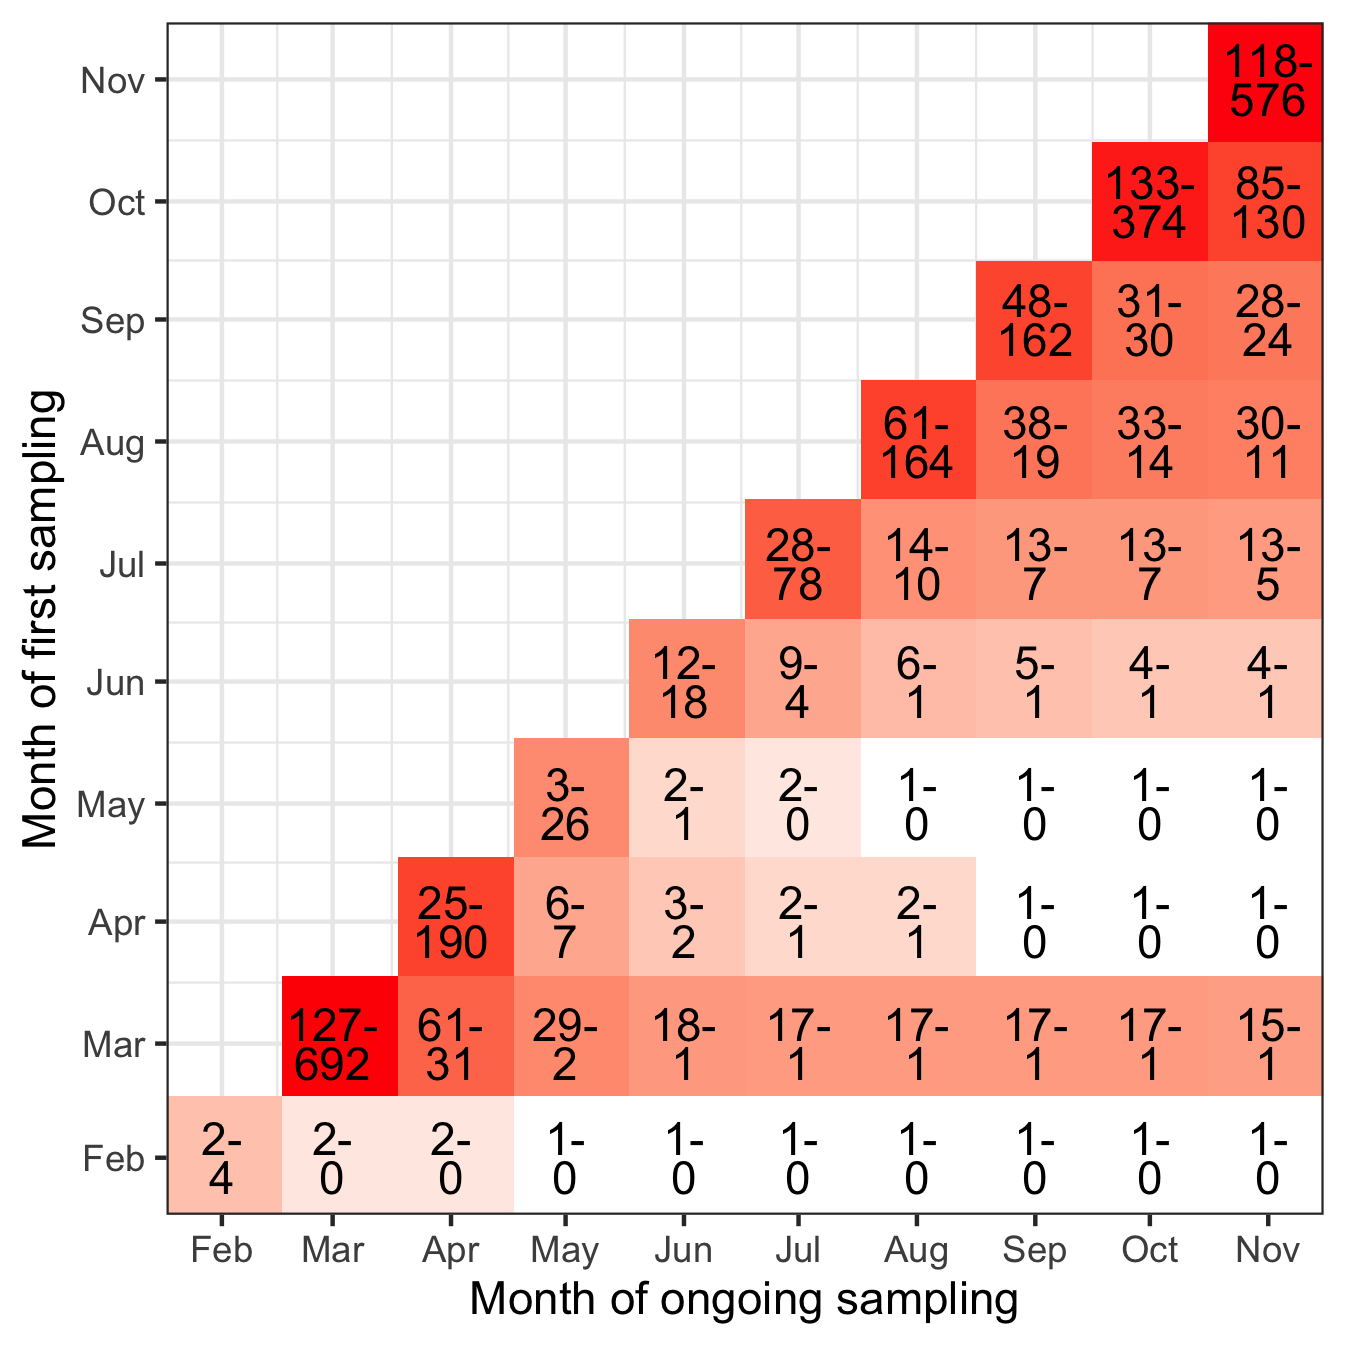
\includegraphics[width=.8\linewidth]{figures/chain_longevity_matrix.png}
\caption{Number of ongoing Swiss transmission chains by the month they were fist sampled. Estimate ranges are between analyses assuming the minimum and maximum plausible number of transmission chains in total. Darker red squares have a higher number of ongoing transmission chains, averaged over the two analyses.}
\label{fig:chain-longevity}
\end{figure}

% \begin{figure}[tbhp]
% \centering
% 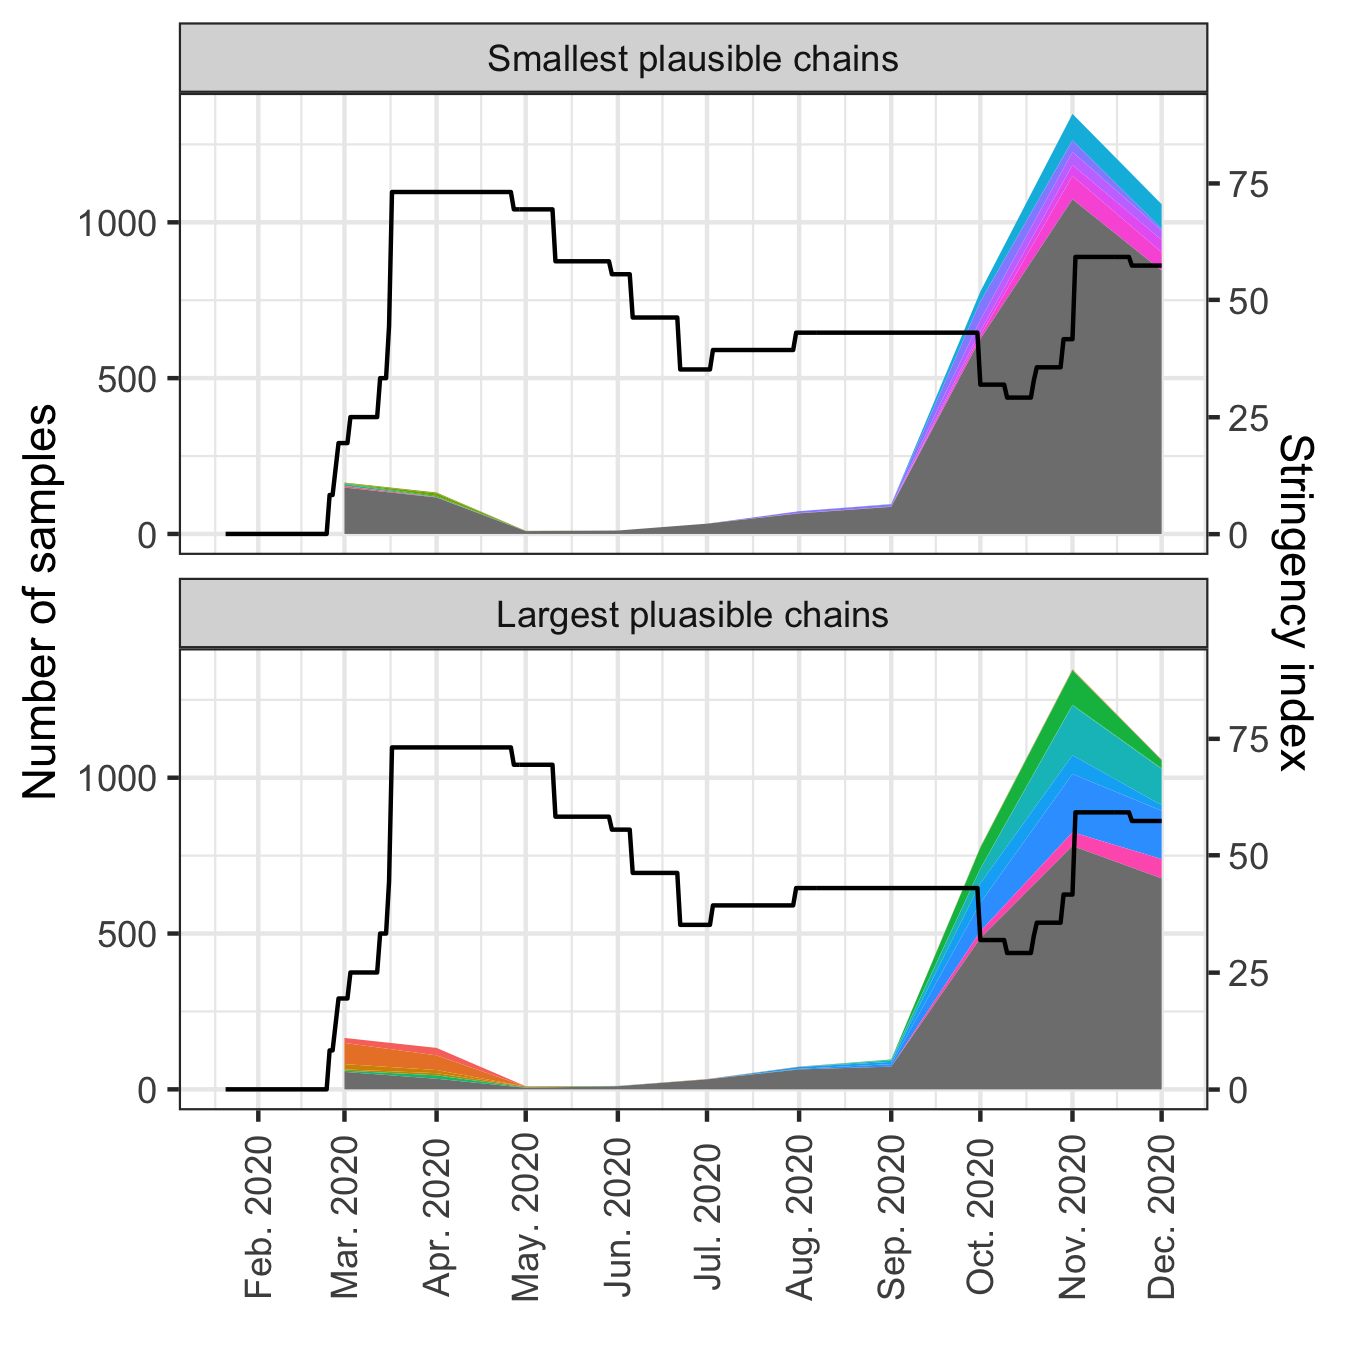
\includegraphics[width=.8\linewidth]{figures/fig_1_chains_through_time.png}
% \caption{Size of sampled Swiss transmission chains through time, compared with the Oxford COVID-19 Government Response Tracker stringency index provided by https://ourworldindata.org/grapher/covid-stringency-index. The \textcolor{red}{N} largest transmission chains during each epidemic wave are highlighted.}  
% \label{fig:chain-sizes}
% \end{figure}

\subsection{Effect of non-pharmaceutical interventions to break transmission chains}

\begin{itemize}
    \item Spike and slab prior for Re multiplier
    \item Bounded time-frame for Re multiplier
    \item Sampling proportion upper bound 0.01 instead of 0.1 - Tim will rerun
    \item Prior on cluster origins is not unique to each cluster, it's a big lognormal blob throughout 2020 - Tim will switch to unif(Jan 1 - Dec 31) so that our prior assumption is that the rate of introductions is constant from when the pandemic started spreading internationally until end of sampling period
    \item How indep are Re estimates from phylo when I select seqs based on conf case \#s? - Tanja's not concerned, the genomes can still tell us what they tell us within what we already know from cases
    \item 50\% prior y/n need Re factor, if y then unif(0, 1) on the factor 
    \item Tim puts independent spike & slab priors in spring, summer, and fall and infers three Re reduction factors so we can see if Summer is really different
    \item Remember Re plot is now background Re (without contact tracing) and no longer the actual average Re
    \item What is the timescale? Does this explain the spike? A: 1 week
\end{itemize}

\section{Discussion}

\section{Materials and methods}
\subsection{Swiss genome sequencing}
Most of the Swiss SARS-CoV-2 genome samples analyzed were provided by Viollier AG, a Swiss medical diagnostics company. RNA was extracted from patient naso- or oral-pharangeal swabs using either the Abbott m2000sp or Seegene STARMag 96x4 Universal Cartridge RNA extraction kit. One aliquot of RNA extract was used for a qPCR test by Viollier and the remaining material from PCR-positive samples was transferred to the Genomics Facility Basel for whole-genome sequencing. Amplicon sequencing was performed using the ARCTIC v3 primer scheme, which yields tiled amplicons of approximately 400bp (12). Libraries were sequenced on an Illumina MiSeq machine, resulting in 2 x 251 base reads. We used V-pipe (13) for raw read quality control, mapping to the reference genome MN908947.3, and consensus base calling. Positions with <5x coverage were not called and positions with >5\% minor base composition were assigned the appropriate ambiguity code. We rejected samples where <90\% of quality-controlled reads did not map to the reference or with < 20,000 bases called. The consensus sequences we generated have been made publicly available on both GISAID (Accession IDs are given in Table S1) and ENA (samples are registered under study PRJEB38472).

We supplemented our Swiss data with other Swiss sequences and foreign sequences available via the “nextfasta” downloaded resource on GISAID (accessed 10. October 2020). We removed non- human samples, duplicates, samples lacking a complete date specification, and samples with sequencing issues flagged by the Nextstrain team (14). We aligned the sequences to the reference genome MN908947.3 using MAFFT. We retained all Swiss sequences 320 kbases long and foreign sequences 327 kbases long. We then masked sites with high homoplasy or other known problems (15, 16). Finally, we used the Nextstrain diagnostic script to additionally exclude sequences with unexpectedly high divergence from the reference, clusters of SNPs in close proximity, or >3000 missing bases (criterion relaxed to >10000 missing bases for Swiss sequences). Sequence counts after each quality-control step are given in Table S2.

\subsection{Sampling procedure}

We considered three genome sample sets: (i) a ``Swiss dataset" of Swiss genomes down-sampled to maximum \maxsamplingpercent\% of confirmed cases each week from \mindate\ to \maxdate, (ii) a ``similarity dataset" with the most genetically similar foreign genomes, and (iii) a ``travel context dataset" with foreign genomes chosen proportionally to monthly incidence- and travel-based estimates of SARS-CoV-2 imports.  

% describe representativeness of Swiss dataset here?
The Swiss dataset was stratified by PANGO lineage, as provided by GISAID. Genome samples from lineages where $>50$\% of genomes on GISAID as of \GISAIDpulldate\ were Swiss were aggregated into higher-level lineages until $>50$\% of the samples were foreign. This aims to ensure each analyzed lineage originated outside of Switzerland.

% describe nextstrain priority protocol for sim dataset
To generate the similarity dataset, we used the Nextstrain priority protocol to choose \gensimscalefactor\ times as many most genetically similar foreign genomes as Swiss genomes for each PANGO lineage. 

% describe context set estimation
To generate the context dataset, we selected \travelcontextscalefactor\ times as many foreign genomes as Swiss genomes proportionally to monthly incidence- and travel-based estimates of SARS-CoV-2 imports and irregardless of PANGO lineage. Estimated introductions were based on case exposure locations recorded by the Swiss Federal Office for Public Health (FOPH), data on tourist arrivals at hotels published by the Swiss Federal Statistical Office (FSO), and data on the number of cross-border commuter permit holders published by the FSO. Here we aim to construct a reasonable prior estimate for monthly imports into Switzerland and recognize that these estimates are sensitive to our subjective weighting of various data sources. Therefore, we interpret our geographic inferences in the context of these assumptions.

Given our estimates for monthly SARS-CoV-2 imports, we randomly selected genomes available on GISAID as of \GISAIDpulldate\ proportional to these estimates. For months without enough genomes from a country, we took extra sequences from the following month if possible and the preceding month if necessary. 

% describe sensitivity analyses here
% We applied this sub-sampling protocol three times with different random seeds. As an additional sensitivity check, we also padded the estimated imports per country and month by 1 before determining the number of context sequences to take. Based on the padded numbers, we randomly chose another set of context sequences. In all, we analyzed three replicate context datasets and one context dataset based on padded imports. In the main text, we discuss results based on only one of the replicate datasets; results from the other datasets are qualitatively similar (Fig. S8 – S10).

% summarize the sample set
The final dataset includes \nswissseqs\ Swiss sequences, \nsimseqs\ genetically similar sequences, and \ntravelseqs\ travel context sequences.

\subsection{Timetree generation}
We stratified the full dataset of Swiss, similarity, and travel genomes by PANGO lineage and built a separate maximum-likelihood phylogeny for each lineage - similar to \cite{DuPlessis2020} - using IQ-TREE \cite{Nguyen2014} with an HKY substitution model, empirical base frequencies, and 4 gamma rate categories. We then rooted each phylogeny with \outgroupisl\ as an outgroup and estimated branch lengths in time-units using least-squares dating (22) with a strict molecular clock and a minimum mutation rate of 0.0008 substitutions/site/year. We additionally assumed the root date to be between 15. Nov. and 24. Dec. 2019 (roughly in line with estimates provided by (23)) and set the minimum branch length to zero. Sequences that violated the strict clock assumption (z-score threshold > 3) were removed and near-zero branches ($<$1.7x10-5 substitutions/site/year) were collapsed into polytomies, reflecting the fact that the sequence data is not sufficient to resolve the ordering of these transmission events. Given the root date constraints, the mutation rate conformed to the lower bound of 0.0008 with extremely narrow confidence intervals. Confidence intervals for node dates were generated in LSD by re- sampling branch lengths 100 times under a lognormal relaxed clock model with standard deviation 0.4.

\subsection{Phylogenetic analyses}
\subsubsection{Transmission chain estimation}
In the tree based on sequences from the Swiss, similarity, and travel context datasets we define Swiss transmission chains as maximal sets of at least 2 Swiss sequences satisfying the following criteria: the Swiss sequences are part of a clade in the tree and the subtree spanned by these Swiss sequences is monophyletic upon removing (a) up to 3 export events where (b) only one export event may occur along each internal branch. Exports are defined to be clades containing non-Swiss sequences. We chose a conservative value for criterion (b) while still allowing some export events and note that the number of inferred transmission chains is robust to different values for criterion (a) given criterion (b) (Fig. S13).
We repeated our analysis interpreting polytomies in two ways. Once, we split Swiss clades descending from polytomies unless the polytomy only had a single non-Swiss descendent (see criterion (b)). Alternatively, we aggregated all Swiss clades descending from polytomies into a single transmission chain. These procedures represent two plausible extremes, the first being maximum introductions and minimum local transmission and the second being minimum introductions and maximum local transmission.
We refer to any Swiss sequence not falling into a Swiss transmission chain as a Swiss singleton. We assume each singleton and each transmission chain represent an independent introduction of SARS-CoV-2 into Switzerland; together these are called Swiss introductions.

\subsubsection{Transmission chain origin estimation}
We inferred the source location of each introduction with a parsimony-based approach. For this, we used only tips in the context dataset and ignored tips in the similarity dataset. Otherwise, over-sequenced locations would show up too often as sources (24). Our procedure is as follows: we begin by labelling the MRCAs of Swiss transmission chains and all subtending nodes in the tree (excepting exported clades) as Swiss. Switzerland was excluded as a possible location for all other nodes. Given these constraints, we calculate the parsimony score for each possible location at each remaining node. Among the possible locations, we also include a “dummy” location to record the maximum parsimony score. So, in a first step we calculate parsimony scores up the tree. In a second step, we covert the parsimony scores at each node to location weights by taking the difference to the “dummy” score. Thus, locations with no support in the subtending tree are given a weight 0 and supported locations are weighted by the number of location changes they prevent. Importantly, these weights are determined through the parsimony score of the subtree descending the considered node and not of the full tree. Finally, we normalized the scores to 1 for each node. In summary, locations that would require more state changes in the subtending tree are down-weighted. For the summary figure Fig. 2b, we conservatively count each polytomy with Swiss descendants as a single introduction.

\subsubsection{Test for travel quarantine effect}

\subsection{Phylodynamic analysis}

We jointly inferred the effective reproductive number and the sampling proportion from all clusters as in (25). We perform inference using the BDSKY model (26) in BEAST2 (27), which assumes a birth- death population dynamical model. Each cluster is assumed to result from an independent birth- death process having its own start time, but sharing all other parameters with the processes associated with the other clusters. We fixed the expected become-uninfectious rate to 36.5 per year, which corresponds to an average time to becoming uninfectious of 10 days. We assumed an HKY (28) nucleotide substitution model with 4 gamma rate categories to account for site-to-site rate heterogeneity (29). We assumed a strict clock with a rate fixed to 8x10-4 substitutions per site per year. The effective reproductive number (Fig. 4a) and the sampling proportion (Fig. 4b) were allowed to vary in a piecewise-constant fashion in intervals of 1 week. An independent smoothing prior was applied to the natural logarithm of each of these time-varying parameters (30). So as to constrain both the relative sizes of the change between weeks and the absolute reproductive number and sampling proportion values, we used smoothing priors formulated as the product between a) a Gaussian penalty on the differences between the logarithm of values for adjacent weeks and b) a function of the value taken in each week. For this function, we used the probability density of a LogNormal(0.8, 0.5) distribution in the case of the Re values, and the density of a Beta(1, 99) distribution in the case of the sampling proportion values. An Exp(1) hyperprior was applied to the variance of the Gaussian component of each smoothing prior.

\section{Acknowledgments}



% \subsection*{Submitting Manuscripts}

% All authors must submit their articles at \href{http://www.pnascentral.org/cgi-bin/main.plex}{PNAScentral}. If you are using Overleaf to write your article, you can use the ``Submit to PNAS'' option in the top bar of the editor window. 

% \subsection*{Format}

% Many authors find it useful to organize their manuscripts with the following order of sections;  title, author line and affiliations, keywords, abstract, significance statement, introduction, results, discussion, materials and methods, acknowledgments, and references. Other orders and headings are permitted.

% \subsection*{Manuscript Length}

% A standard 6-page article is approximately 4,000 words, 50 references, and 4 medium-size graphical elements (i.e., figures and tables). The preferred length of articles remains at 6 pages, but PNAS will allow articles up to a maximum of 12 pages.

\subsection*{References}
\printbibliography

% References should be cited in numerical order as they appear in text; this will be done automatically via bibtex, e.g. \cite{belkin2002using} and \cite{berard1994embedding,coifman2005geometric}. All references cited in the main text should be included in the main manuscript file.

% \subsection*{Data Archival}

% PNAS must be able to archive the data essential to a published article. Where such archiving is not possible, deposition of data in public databases, such as GenBank, ArrayExpress, Protein Data Bank, Unidata, and others outlined in the \href{https://www.pnas.org/page/authors/journal-policies#xi}{Information for Authors}, is acceptable.

% \subsection*{Language-Editing Services}
% Prior to submission, authors who believe their manuscripts would benefit from professional editing are encouraged to use a language-editing service (see list at www.pnas.org/page/authors/language-editing). PNAS does not take responsibility for or endorse these services, and their use has no bearing on acceptance of a manuscript for publication. 

% \begin{figure}%[tbhp]
% \centering
% 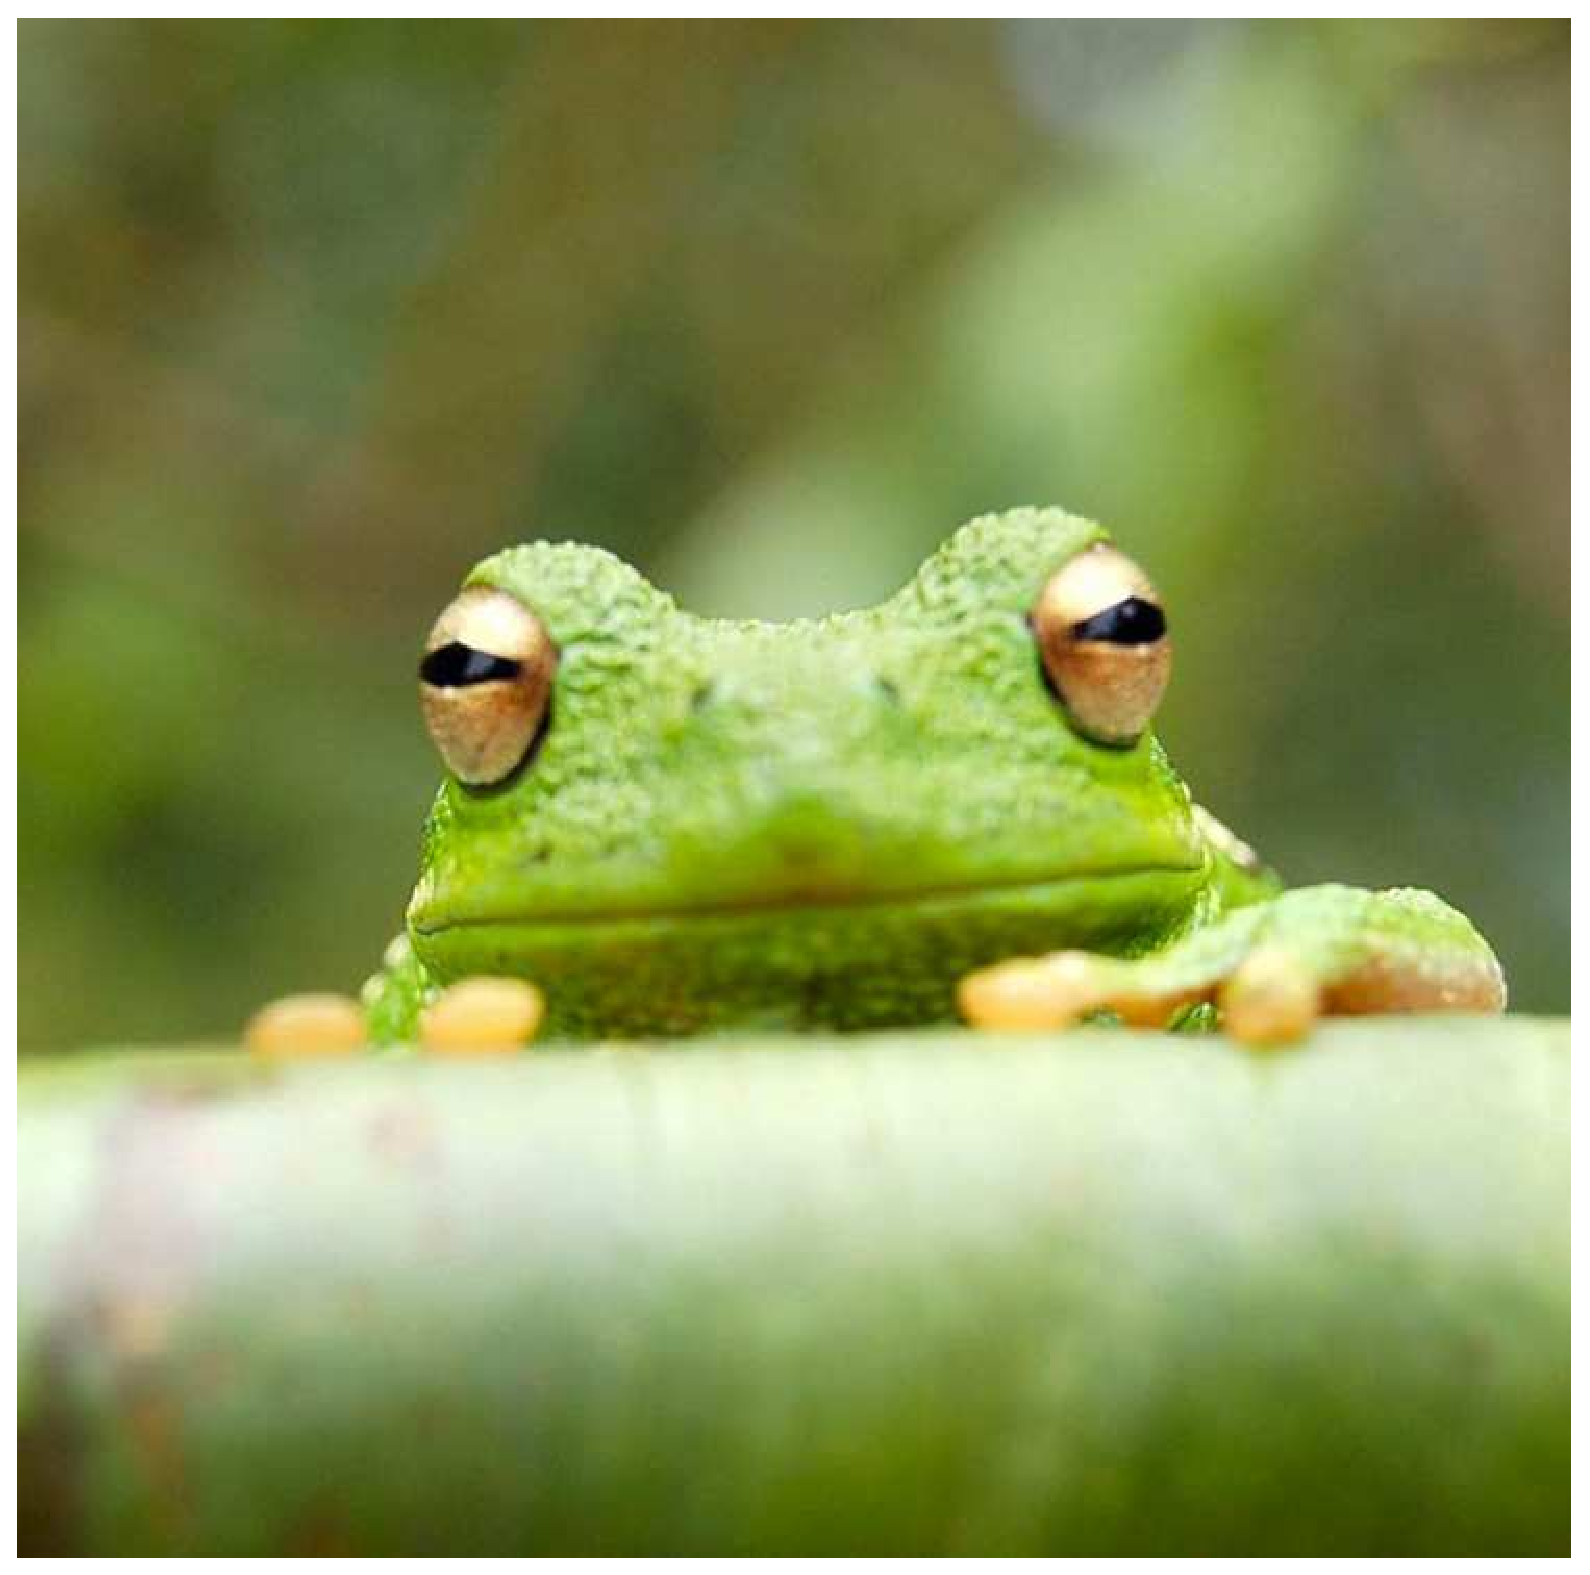
\includegraphics[width=.8\linewidth]{frog}
% \caption{Placeholder image of a frog with a long example legend to show justification setting.}
% \label{fig:frog}
% \end{figure}


% \begin{SCfigure*}[\sidecaptionrelwidth][t]
% \centering
% 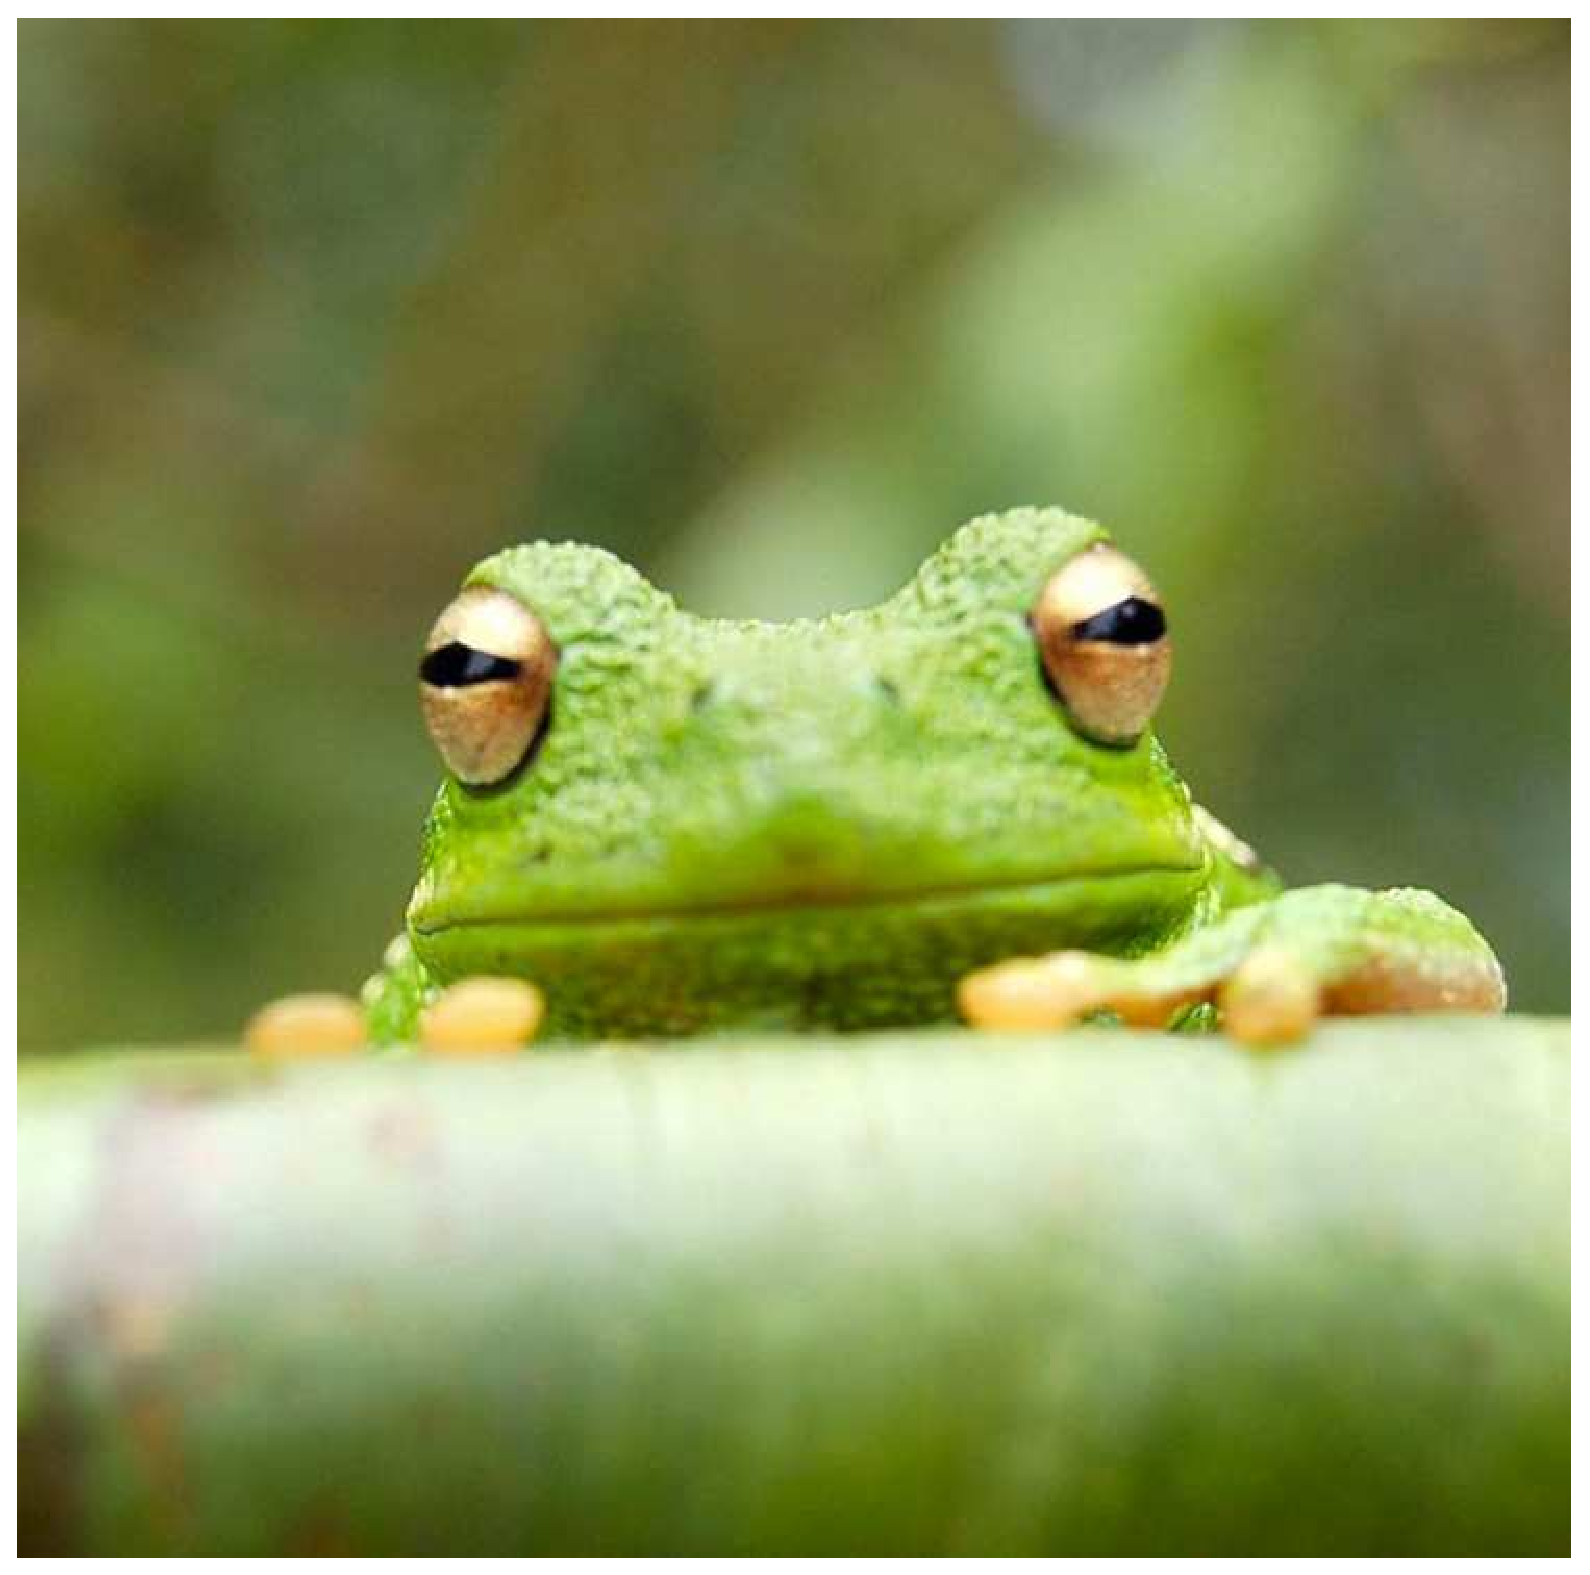
\includegraphics[width=11.4cm,height=11.4cm]{frog}
% \caption{This legend would be placed at the side of the figure, rather than below it.}\label{fig:side}
% \end{SCfigure*}

% \subsection*{Digital Figures}

% EPS, high-resolution PDF, and PowerPoint are preferred formats for figures that will be used in the main manuscript. Authors may submit PRC or U3D files for 3D images; these must be accompanied by 2D representations in TIFF, EPS, or high-resolution PDF format. Color images must be in RGB (red, green, blue) mode. Include the font files for any text.

% Images must be provided at final size, preferably 1 column width (8.7cm). Figures wider than 1 column should be sized to 11.4cm or 17.8cm wide. Numbers, letters, and symbols should be no smaller than 6 points (2mm) and no larger than 12 points (6mm) after reduction and must be consistent. 

% Figures and tables should be labelled and referenced in the standard way using the \verb|\label{}| and \verb|\ref{}| commands.

% Figure \ref{fig:frog} shows an example of how to insert a column-wide figure. To insert a figure wider than one column, please use the \verb|\begin{figure*}...\end{figure*}| environment. Figures wider than one column should be sized to 11.4 cm or 17.8 cm wide. Use \verb|\begin{SCfigure*}...\end{SCfigure*}| for a wide figure with side legends.

% \subsection*{Tables}
% Tables should be included in the main manuscript file and should not be uploaded separately.

% \subsection*{Single column equations}

% Authors may use 1- or 2-column equations in their article, according to their preference.

% To allow an equation to span both columns, use the \verb|\begin{figure*}...\end{figure*}| environment mentioned above for figures.

% Note that the use of the \verb|widetext| environment for equations is not recommended, and should not be used. 

% \begin{figure*}[bt!]
% \begin{align*}
% (x+y)^3&=(x+y)(x+y)^2\\
%       &=(x+y)(x^2+2xy+y^2) \numberthis \label{eqn:example} \\
%       &=x^3+3x^2y+3xy^3+x^3. 
% \end{align*}
% \end{figure*}


% \begin{table}%[tbhp]
% \centering
% \caption{Comparison of the fitted potential energy surfaces and ab initio benchmark electronic energy calculations}
% \begin{tabular}{lrrr}
% Species & CBS & CV & G3 \\
% \midrule
% 1. Acetaldehyde & 0.0 & 0.0 & 0.0 \\
% 2. Vinyl alcohol & 9.1 & 9.6 & 13.5 \\
% 3. Hydroxyethylidene & 50.8 & 51.2 & 54.0\\
% \bottomrule
% \end{tabular}

% \addtabletext{nomenclature for the TSs refers to the numbered species in the table.}
% \end{table}

% \subsection*{Supporting Information Appendix (SI)}

% Authors should submit SI as a single separate SI Appendix PDF file, combining all text, figures, tables, movie legends, and SI references. SI will be published as provided by the authors; it will not be edited or composed. Additional details can be found in the \href{https://www.pnas.org/authors/submitting-your-manuscript#manuscript-formatting-guidelines}{PNAS Author Center}. The PNAS Overleaf SI template can be found \href{https://www.overleaf.com/latex/templates/pnas-template-for-supplementary-information/wqfsfqwyjtsd}{here}. Refer to the SI Appendix in the manuscript at an appropriate point in the text. Number supporting figures and tables starting with S1, S2, etc.

% Authors who place detailed materials and methods in an SI Appendix must provide sufficient detail in the main text methods to enable a reader to follow the logic of the procedures and results and also must reference the SI methods. If a paper is fundamentally a study of a new method or technique, then the methods must be described completely in the main text.

% \subsubsection*{SI Datasets} 

% Supply .xlsx, .csv, .txt, .rtf, or .pdf files. This file type will be published in raw format and will not be edited or composed.


% \subsubsection*{SI Movies}

% Supply Audio Video Interleave (avi), Quicktime (mov), Windows Media (wmv), animated GIF (gif), or MPEG files. Movie legends should be included in the SI Appendix file. All movies should be submitted at the desired reproduction size and length. Movies should be no more than 10MB in size.


% \subsubsection*{3D Figures}

% Supply a composable U3D or PRC file so that it may be edited and composed. Authors may submit a PDF file but please note it will be published in raw format and will not be edited or composed.


\matmethods{Please describe your materials and methods here. This can be more than one paragraph, and may contain subsections and equations as required. 

\subsection*{Subsection for Method}
Example text for subsection.
}

\showmatmethods{} % Display the Materials and Methods section

\acknow{This work was supported by the Swiss National Science Foundation (SNSF) through grant number 31CA30\_196267 (to TS).
}

\showacknow{} % Display the acknowledgments section

% Bibliography
\bibliography{pnas-sample}

\end{document}
